\documentclass[../Cover.tex]{subfiles}

\begin{document}

\begin{minipage}[t]{0.2\textwidth} 
		
\includegraphics[width=0.8\textwidth]{DC.png}
	% Required Equipment
	\begin{tabular}{p{0.8\textwidth}}
		\small Required Materials \\
		\hline
		\tiny \begin{itemize}
			\item Target type: 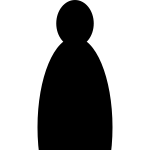
\includegraphics[width=0.15\textwidth]{body-target.png}
			\item 3 rounds 
		\end{itemize}
		\\
	\end{tabular}
\end{minipage}
\hfill
\begin{minipage}[t]{0.8\textwidth}
	\begin{minipage}[t]{0.4\textwidth}
		% EXERCISE NAME
		\begin{tabular}{ p{\textwidth} }			
			\large Failure to Stop Drill\\[0.1\textheight]	
		\end{tabular}
	\end{minipage}
	\hfill
	\begin{minipage}[t]{0.55\textwidth}
		% Basic Info
		\begin{tabular}{ | l | l | l |}
			\hline
			\tiny Weapon Type & \tiny Distance & \tiny Par \\ 
			\hline
			\tiny Any & \tiny 8-10ft & \tiny 4s \\ 
			\hline
		\end{tabular}
	\end{minipage}
	% Steps and Scoring	
	\begin{tabular}{ | p{0.85\textwidth} |}
		\hline
		Steps\\ 
		\hline
		\tiny \begin{enumerate}[topsep=0pt, partopsep=0pt]
			\item Select starting position: low ready, holstered, or tabled.
			\item Wait for a start signal.
			\item Place two shots in the chest of the target. (approx. 8" circle)
			\item Pause. Assess the situation.
			\item Place one shot in the head of the target. (approx. 4" circle)
		\end{enumerate}
		\\ [0.2\textheight]
		\hline
		Scoring \\
		\hline
		\tiny \begin{itemize}[topsep=0pt, partopsep=0pt]
			\item The drill should be completed within 4 seconds.
			\item Failure for shot placement outside of the designated areas.
			\item For an added challenge, start from holstered.
			\item For an added challenge, have a partner call for the final shot.
		\end{itemize}		
		\\ [0.2\textheight]
		\hline
	\end{tabular}
\end{minipage}
\end{document}
